% # -*- coding: utf-8 -*-
\section{Background} \label{seciton:background}

\begin{figure}[t]
  \begin{center}
    \hspace{-5.5ex}
    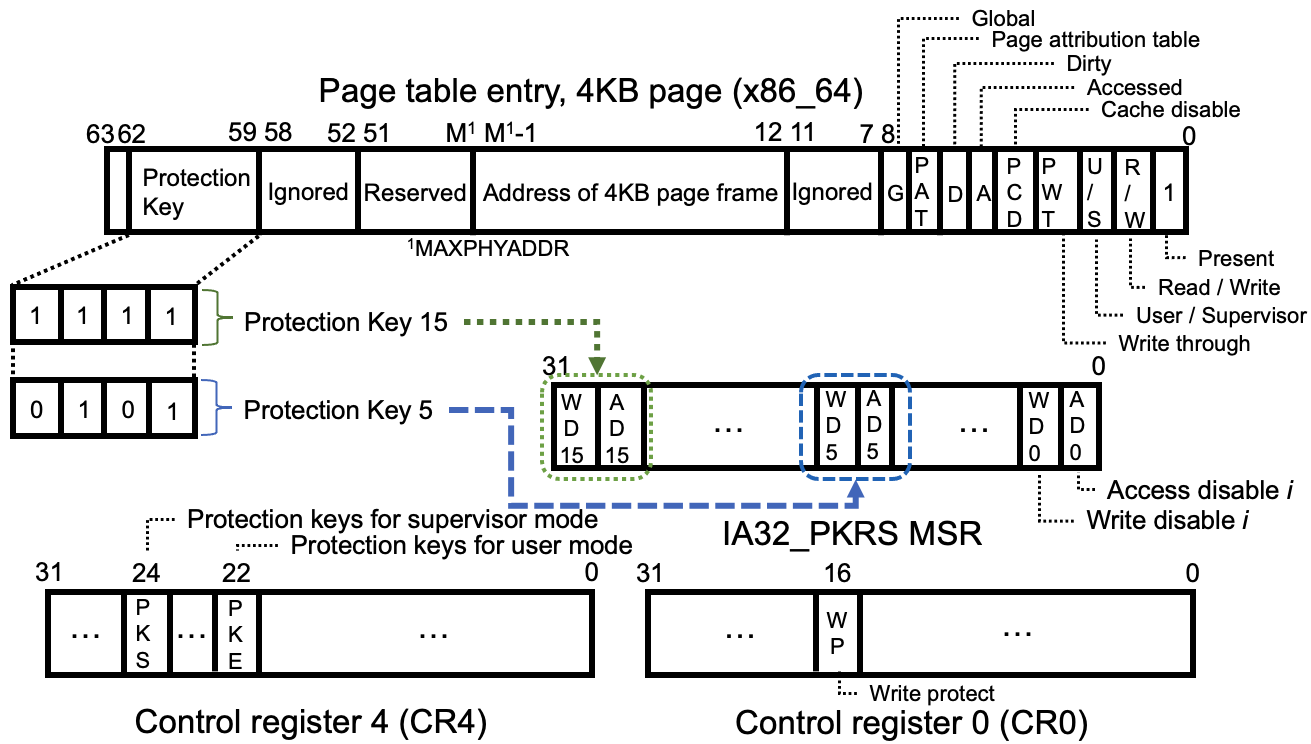
\includegraphics[bb=0 0 1311 744, scale=.200]{./imgs/002_screenshot_2021-07-26_19.13.09.png}
  \end{center}
  %  \vspace{-4.5ex}
% \vspace{-2.0ex}  
  \caption{
    %
    Intel memory protection key \cite{intel-mpk}
    %
  }
%  \vspace{-0.5ex}      
%  \ecaption{
%    Overview of software based side channel attack
%  }
  % \vspace{-3.0ex}
 \label{fig:mpk_overview}
\end{figure}

\subsection{Memory Protection Key}
% MPK は仮想アドレスを構成するPTEに対して読書き権限を操作可能な Intel
% CPU の機能である.\figref{fig:mpk_overview}に示す通り,PKS はカーネル
% モード用の MPK であり,次の機能が提供される\cite{intel-mpk}.
% MPK is an Intel CPU feature that allows manipulation of read permissions for
% PTEs that comprise a virtual address. As shown in \figref{fig:mpk_overview}, PKS
% is the MPK for kernel mode and provides the following functions
% \cite{intel-mpk}.

% \item Protection keys for supervisor(PKS):カーネルモードで利用する
%   Protection keyである.Control register 0(CR0)Write Protect フラグ
%   かつ CR4 PKS フラグにて有効 / 無効を制御する.
%   %
%   PKS では,PTEに対し,4 bit 割当てられ,16 個の Protection key を指定可能である.
%  Protection key 毎の読書き制限(Write
%     disable(WD),Read disable(RD))2 bit 操作のため, 32bitの読書き
%   制限操作レジスタIA32\_PKRS MSRレジスタ(以降,PKRS)をCPUコア毎に備える.

% MPK は Intel CPU の提供するセキュリティ機能であり,仮想記憶空間のペー
% ジ単位(Page Table Entry, PTE)にて読書き制限を制御可能とする \cite{intel-mpk}.
% %
% MPK では,ユーザモードで利用する Protection Keys for Userspace(PKU)と
% 読書き制限操作レジスタ Protection Key Right for User-mode (PKRU),
% ならびにカーネルモードで利用する Protection Keys for Supervisor(PKS)と
% 読書き制限操作レジスタ \verb|IA32_PKRS_MSR| レジスタ(以降,PKRS)がある.

Intel CPU provides an MPK, which is a security feature provided to control read
and write restrictions on a page basis, that is, page table entry (PTE)
\cite{intel-mpk}.
% in virtual memory space 
%
The MPK includes protection keys for userspace (PKU) and the protection key
right for user mode register (hereinafter, PKRU) for the user mode.
% the There are 
In addition, the MPK includes PKS and \verb|IA32_PKRS_MSR| register
(hereinafter, PKRS) for the kernel mode.

%the PTE has a 4-bit protection key (Pkey) for 16 Pkeys, 
As shown in Figure \ref{fig:mpk_overview}, the PTE has 16 4-bit protection keys
(Pkeys), and the 32-bit flag (two bits per Pkey: write disable (WD) and access
disable (AD)) controls the read and write restriction for each Pkey.
% basis via 
% In addition, read restriction is
%
The read and write restriction for Pkey {\it i} ($0 \leq i \leq 15$) is performed via the
register. If the value of bit AD {\it i} $\times$ 2 is 0, read is allowed. In contrast,
if the value of bit AD {\it i} $\times$ 2 is 1, read is not allowed.
% of {\it i} $\times$ 2 is 1, read is disallowed; 
%
Additionally, if the value of bit WD {\it i} $\times$ 2+1 is 0, write is allowed; and if the
value of bit WD {\it i} $\times$ 2+1 is 1, write is not allowed.

In MPK, read and write limits can be controlled separately in the specific
register (e.g., PKRU and PKRS). For multiple PTEs, the read and write
restriction can be controlled by specifying the Pkey.
% collectively using the read restriction operation register by specifying Pkey.




% \figref{fig:mpk_overview}に示す通り,
% %
% PTE において,4 bit の Protection key (Pkey) が割当てられており,16 個
% の Pkey を指定可能である.また,32 bit の読書き制限操作レジスタ(
%   Pkey あたり,Write disable(WD),Access disable(AD)の2 bit)を
% 介して,Pkey 単位で読書き制限の制御を行う.

% %{\it i}番目の
% Pkey {\it i}($0 \leq i \leq 15$)に対する読書き制限制御は,読書き制限
% 操作レジスタを介して行う.
% %
% {\it i} $\times$ 2のビット AD {\it i} の値が1の場合,読込み不可.0の
% 場合,読込み可,{\it i} $\times$ 2+1 のビットWD {\it i}+1が1の場合,
% 書込み不可,0の場合,書込み可とされる.

% MPKにおいて,読書き制限操作レジスタでの読込み制限,書込み制限は個別に
% 制御可能である.
% %
% また,複数のPTEに対して,Pkey を指定することで,読書き制限操作レジスタ
% を利用して一括に読書き制限制御を可能としている.
%
% 従来,PTE単位での読書き制御は読込みのみ,あるいは読書きの2種類を指定で
% きたが,MPKを用いることで読込み制限,書込み制限を個別に制御可能である.
% %
% また,Protection keyを複数のPTEに指定することで,読書き制限操作レジス
% タのみでの一括制御を可能としている.


% \begin{figure}[t]
%   \centering
%   \includegraphics[bb=0 0 1237 862, scale=.200]{./imgs/A01X_09_screen_shot_2021-12-17_15.29.59.png}
%     %  \vspace{-4.5ex}  
%   \caption{
%     %
%     Overview of privilege escalation and DoS
%     %
%   }
%   \label{fig:overview_kvuln}
% %\vspace{-5.0ex}        
% \end{figure}


% \begin{table}[t]
%   \centering
% \caption{
% %
%   %The comparison of feature among Blockchain.info, WalletExplorer.com, Bitiodine, and our proposed system.
%   %
%   Available PoC code for Linux kernel vulnerability list.
%   DoS: denial-of-service, Mem. Corr.: Memory Corruption
%   %among existing systems and proposed system
%   %
%   % CVE-2017-1000112
%   % https://www.exploit-db.com/exploits/43418
%   % CVE-2017-7533
%   % https://www.exploit-db.com/exploits/44302
%   % CVE-2016-9793
%   % https://www.exploit-db.com/exploits/41995
%   % CVE-2016-4997
%   % https://www.exploit-db.com/exploits/40435
% }
% %  \vspace{-0.5ex}  
% \scalebox{1.0}{
% \begin{tabular}{lll}
% %\hline
% \hline \noalign{\smallskip}
% \begin{tabular}{c}
%   {\bf CVE ID}
% \end{tabular}
% &
% \begin{tabular}{c}
%   {\bf Types}
% \end{tabular}
% %& {\bf PoC} & {\bf Publish Date} &
% &
% \begin{tabular}{c}
%   {\bf Description}
% \end{tabular}  
%     \\
%        \noalign{\smallskip}
%        \hline
%        \noalign{\smallskip}
%        CVE-2016-4997\cite{CVE-2016-4997} & DoS, Mem. Corr. & Boundary check error\\% in setsockopt implementation\\
%        CVE-2016-9793\cite{CVE-2016-9793} & DoS, Mem. Corr. & Boundary check error\\% in net/core/sock.c\\
%        CVE-2017-6074\cite{CVE-2017-6074} & DoS & Use after free\\% in net/core/sock.c\\                     
%        CVE-2017-7533\cite{CVE-2017-7533} & DoS, Mem. Corr. & Race condition\\% in the fsnotify implementation \\
%        CVE-2017-16995\cite{CVE-2017-16995} & DoS, Mem. Corr. & Boundary check error\\% in kernel/bpf/verifier.c\\% occurs memory corruption.\\
%        CVE-2017-1000112\cite{CVE-2017-1000112} & Mem. Corr. & Race condition\\% in net/ipv4/ip\_output.c\\

% \hline
% \end{tabular}
% }
% \label{tb:kernel_vulnerability_list}
% %\vspace{-1.0ex}  
% \end{table}


% \begin{figure*}[t]
%   \begin{center}
%     %\includegraphics[bb=0 0 1254 835, scale=.240]{./imgs/003_screen_shot_2019-08-14_17.12.23.png}
%     \includegraphics[bb=0 0 1581 882, scale=.240]{./imgs/A01X_01_screenshot_2021-09-17_21.18.21.png}
%   \end{center}
% %  \vspace{-1.0ex}
%   \caption{
%     %
%     Overview of the vulnerable kernel code tracer (vkTracer)
%     %
%   }
% %  \vspace{-2.0ex}
%   %\label{fig:restriction_approach_applying}
%   \label{fig:approach_overview}
% %  \vspace{-2.0ex}
% \end{figure*}



\subsection{Kernel Vulnerability}
% カーネル脆弱性は,カーネルへの攻撃に利用可能とされる実装不備とされる
% \cite{chen11linux}.
% %
% 特権奪取攻撃では,カーネル脆弱性を利用して任意のコードを挿入し,カーネ
% ルにおける権限操作を行うカーネル関数\verb|commit_creds| および
% \verb|prepare_kernel_cred|の呼出しによる権限情報の変更
% \cite{CVE-2016-4997,CVE-2016-9793,CVE-2017-1000112},または,カーネル
% 仮想記憶空間上の権限情報を格納するカーネルデータの変数\verb|cred|を改
% ざんし,ユーザプロセスのユーザIDを管理者ユーザへ変更する
% \cite{CVE-2017-16995}.

% 特権昇格攻撃,およびカーネルの提供するセキュリティ機能に対する無効化攻撃では,
% カーネルへの攻撃に利用可能とされる実装不備であるカーネル脆弱性のなかでも,カーネ
% ル脆弱性を介した任意のカーネルコードの挿入,実行によるメモリ破壊攻撃が利用される
% \cite{chen11linux}

% Linux カーネルにおいて,全てのユーザプロセスは同一のカーネルの仮想記憶空間を利用
% している.攻撃の起点となるカーネル脆弱性と共通の仮想記憶空間に存在するカーネル
% コード,およびカーネルデータは,仮想アドレスを指定し参照可能であり,メモリ破壊攻
% 撃に成功した場合,任意のカーネルデータは改ざん可能となる.
% %
% In the Linux kernel, all user processes use the same kernel virtual memory
% space. The kernel code and kernel data in the virtual memory space common to the
% kernel vulnerability that is the starting point of the attack can be referenced
% by specifying a virtual address, and the memory corruption attack If the attack
% succeeds, any kernel data can be tampered with.

%Kernel vulnerabilities are types of improper implementations that lead to kernel
Kernel vulnerabilities are improper implementations that lead to kernel attacks
\cite{chen11linux}. 
%
Table \ref{tb:kernel_vulnerability_cwe_list} shows the Common Weakness Enumeration
(CWE) ranking for CWE of kernel memory vulnerability. CWE represents the
categorized software and hardware weakness type. 
%
Table \ref{tb:kernel_vulnerability_cwe_list} indicates a running kernel can be
damaged in a variety of ways through a kernel vulnerability attack. 
% 
%
Additionally, Proof of Concept (PoC) codes that achieve the Linux kernel
compromising for specific CVE. Table \ref{tb:kernel_vulnerability_cwe_list}
indicates 27 PoC codes of kernel memory vulnerability are available in the
Exploit Database \cite{exploitdb}. 
%A lot of PoC codes are widely provided 

%
% for each CWE.

%
% 特権昇格攻撃では,カーネルにおける権限操作を行うカーネル関数を強制的に呼出し,権
% 限情報が変更される \cite{CVE-2016-4997,CVE-2016-9793,CVE-2017-1000112}.また,権
% 限情報を格納するカーネルデータの変数 \verb|cred| を改ざんし,ユーザプロセスのユーザ ID
% を管理者ユーザへ変更する \cite{CVE-2017-16995}.
% perform the modification
To investigate which CVE are reproducible, PoC codes are introduced from CWE
ranking (Table \ref{tb:kernel_vulnerability_cwe_list}).
Table \ref{tb:kernel_vulnerability_poc_list} shows the result of four PoC codes are
reproducible and can compromise the environment for Linux kernel.
%
Three PoC codes forcibly invokes kernel codes that modify privileged information
to achieve the privilege escalation
\cite{CVE-2016-4997,CVE-2016-9793,CVE-2017-1000112}. 
%
% privilege operations in the kernel and 
% Specifically, other 
One PoC code overwrites the variable \verb|cred| of the
kernel data that stores privileged information from the normal user to the
administrator \cite{CVE-2017-16995}.
% with, and 
%
% セキュリティ機能である強制アクセス制御の無効化攻撃では,カーネルにおける強制アク
% セス制御を管理する関数ポインタの一覧\verb|selinux_hooks|の一部を強制アクセス制御
% を回避するカーネル関数へのポインタへ変更し,セキュリティ機能の無効化を行う
% \cite{nexus5exploit,grsecurity}.
% %
% 強制アクセス制御が無効化された場合,管理者権限の制限は行われない.特権奪取攻撃と
% 組み合わせることで,管理者権限を自由に利用可能となる.
% In the attack to security feature, 
The defeat of the MAC forcefully modifies the list of function pointers that
manage the access control decisions in the kernel. Meanwhile, the variable
\verb|selinux_hooks|, which stores function pointers, is modified to the inserted
kernel 
%are changed to inserted kernel
codes that bypass the access control \cite{nexus5exploit,grsecurity}.
% , thereby disabling the security feature

% When the mandatory access control is disabled, no restrictions for
% administrative privilege. 
Therefore, the combination of privilege escalation and the MAC being disabled
provides full administrator capability to the adversary with no restrictions on
the kernel.
%achieves 
% lead 
% privileges can be used freely.
\begin{table}[t]
    \centering
    %\caption{Chen らによるカーネルの脆弱性を用いた攻撃の影響種別 \cite{chen11linux}}
    %\caption{Affection of kernel vulnerability attack \cite{chen11linux}.}
    \caption{Top CWE of kernel memory vulnerability \cite{nvd} %\cite{chen11linux}
    }
    % ($\checkmark$ is supported; $\triangle$ is partially supported)}
    \scalebox{0.62}{  
    \begin{tabular}{llcc}
      %  \hline
        \hline \noalign{\smallskip}
      %  \hline
      \begin{tabular}{c}
        {\bf Type}
      \end{tabular}
      &
      \begin{tabular}{c}
        {\bf Content}
      \end{tabular}
      &
      \begin{tabular}{c}
        {\bf CVE}
      \end{tabular}
      &
      \begin{tabular}{c}
        {\bf PoC}
      \end{tabular}
      \\
       %影響                  & 内容\\
    %    Types             & Content & CVE & PoC\\
       \hline \noalign{\smallskip}
      %  \hline
      CWE-200 	& Exposure of Sensitive Information to an Unauthorized Actor	&125	&6\\
      NVD-CWE-Other 	& Other	&87	&5\\
      CWE-119 	&Improper Restriction of Operations within the Bounds of a Memory Buffer	&82	&3\\
      CWE-401 	&Missing Release of Memory after Effective Lifetime	&78	&0\\
      CWE-399 	&Resource Management Errors	&52	&1\\
      CWE-20 	&Improper Input Validation	&44	&1\\
      CWE-787 	&Out-of-bounds Write	&31	&1\\
      CWE-416 	&Use After Free	&20	&0\\
      CWE-125 	&Out-of-bounds Read	&19	&1\\
      %CWE-362 	&Concurrent Execution using Shared Resource with Improper Synchronization ('Race Condition')	&18	&3\\
      CWE-362 	&Concurrent Execution using Shared Resource ('Race Condition')	&18	&3\\
      CWE-189 	&Numeric Errors	&17	&0\\
      CWE-264 	&Permissions, Privileges, and Access Controls	&17	&2\\
      CWE-190 	&Integer Overflow or Wraparound	&16	&0\\
      CWE-909 	&Missing Initialization of Resource	&14	&0\\
      CWE-400 	&Uncontrolled Resource Consumption	&12	&0\\
      CWE-772 	&Missing Release of Resource after Effective Lifetime	&11	&0\\
      NVD-CWE-noinfo 	&Insufficient Information	&11	&1\\
      \hline \noalign{\smallskip}
      Other CWE & Under 10 CVE & 70&3\\
      \hline \noalign{\smallskip}
      Total & & 724 & 27\\
      \hline \noalign{\smallskip}
    %   \hline

    %    Obtain Information & Information leakage from kernel & $\triangle$\\
    %    Gain Privilege & Taking of administrator privilege   & $\checkmark$\\
    %    Bypass a Restriction & Evading of access control decision & $\checkmark$\\
    %    Overflow & Overwriting of stack or heap region & $\checkmark$\\
    %    Denial of Service & Forcing kernel to stop running & $\checkmark$\\
    %    Memory Corruption & Overwriting or reading of kernel code / data on virtual memory & $\checkmark$\\
      %  Memory corruption  & Overwriting or reading of kernel code / data on virtual memory & $\checkmark$\\
      %  Policy violation   & Miss implementation of access control decision & $\checkmark$\\
      %  Denial of Service  & Forcing kernel to stop running & $\checkmark$\\
      %  OS information leakage  & Information leakage from uninitialized data variables & $\triangle$\\
    %    \hline
    \end{tabular}
  }
    \label{tb:kernel_vulnerability_affection}
  \end{table}
  
  \begin{table}[t]
    \centering
  \caption{
  %
    %The comparison of feature among Blockchain.info, WalletExplorer.com, Bitiodine, and our proposed system.
    %
    % Available PoC code for Linux kernel memory vulnerability list
    Executable PoC code for Linux kernel memory vulnerability list
    ($\checkmark$ is protection available;)
    % $\triangle$ is partially supported)
    % DoS: Denial of Service, Mem. Corr.: Memory Corruption
    %among existing systems and proposed system
    %
    % CVE-2017-1000112
    % https://www.exploit-db.com/exploits/43418
    % CVE-2017-7533
    % https://www.exploit-db.com/exploits/44302
    % CVE-2016-9793
    % https://www.exploit-db.com/exploits/41995
    % CVE-2016-4997
    % https://www.exploit-db.com/exploits/40435
  }
  %  \vspace{-0.5ex}  
  \scalebox{0.75}{
  \begin{tabular}{lllc}
  %\hline
  \hline \noalign{\smallskip}
  \begin{tabular}{c}
    {\bf CVE ID}
  \end{tabular}
  &
  \begin{tabular}{c}
    {\bf CWE}
  \end{tabular}
  &
%   \begin{tabular}{c}
%     {\bf Types}
%   \end{tabular}
  %& {\bf PoC} & {\bf Publish Date} &
%   &
  \begin{tabular}{c}
    {\bf Description}
  \end{tabular}  
  &
  \begin{tabular}{c}
    {\bf KDPM}
  \end{tabular}  
      \\
         \noalign{\smallskip}
         \hline
         \noalign{\smallskip}
         CVE-2016-4997\cite{CVE-2016-4997} & CWE-264 & Boundary check error in setsockopt function & $\checkmark$\\
         CVE-2016-9793\cite{CVE-2016-9793} & CWE-119 & Boundary check error in net/core/sock.c & $\checkmark$\\
        %  CVE-2017-6074\cite{CVE-2017-6074} & & DoS & Use after free\\% in net/core/sock.c\\                     
        %  CVE-2017-7533\cite{CVE-2017-7533} & DoS, Mem. Corr. & Race condition\\% in the fsnotify implementation \\
         CVE-2017-16995\cite{CVE-2017-16995} & CWE-119 & Boundary check error in kernel/bpf/verifier.c & $\checkmark$\\
         % occurs memory corruption.\\
         CVE-2017-1000112\cite{CVE-2017-1000112} & CWE-362 & Race condition in net/ipv4/ip\_output.c & $\checkmark$\\

        %  CVE-2016-4997\cite{CVE-2016-4997} & CWE-264 & DoS, Mem. Corr. & Boundary check error in setsockopt function\\
        %  CVE-2016-9793\cite{CVE-2016-9793} & CWE-119 & DoS, Mem. Corr. & Boundary check error in net/core/sock.c\\
        % %  CVE-2017-6074\cite{CVE-2017-6074} & & DoS & Use after free\\% in net/core/sock.c\\                     
        % %  CVE-2017-7533\cite{CVE-2017-7533} & DoS, Mem. Corr. & Race condition\\% in the fsnotify implementation \\
        %  CVE-2017-16995\cite{CVE-2017-16995} & CWE-119 & DoS, Mem. Corr. & Boundary check error in kernel/bpf/verifier.c\\% occurs memory corruption.\\
        %  CVE-2017-1000112\cite{CVE-2017-1000112} & CWE-362 & Mem. Corr. & Race condition in net/ipv4/ip\_output.c\\  
  \hline \noalign{\smallskip}         
%   \hline
  \end{tabular}
  }
\label{tb:kernel_vulnerability_list}
\end{table}


% Kernel misimplementations result in kernel vulnerabilities, which can
% eventually lead to kernel attacks \cite{chen11linux}.
% %
% A kernel attack can lead to several types of damages to the running
% kernel.
% %
% Figure \ref{fig:overview_kvuln} shows that typical attacks include privilege
% escalation through memory corruption, which can lead to administrator privileges
% (e.g., root account) and DoS through unusual kernel data modification, defeating
% the stability of the kernel \cite{chen11linux}.

% \subsection{PoC Codes}
% %
% Several kernel vulnerabilities have been reported for Linux kernels
% \cite{cvedetails}.
% %
% PoC codes are small programs that directly invoke
% vulnerable kernel codes to exploit a known vulnerability.
% %
% Table \ref{tb:kernel_vulnerability_list} summarizes some of the available PoC
% codes. These include the execution techniques to invoke vulnerable kernel code
% in a specific version of the Linux kernel.
% %
% In this study, several kernel vulnerabilities are applied for the
% evaluation of vkTracer:

% \begin{itemize}

% %\item {\bf Memory corruption}: This overwrites the memory region of the
% \item {\bf Privilege escalation}: This overwrites credential
%   information through the corruption of stack or heap areas
%   and exploits a kernel vulnerability to achieve privilege
%   escalation.
%   %or defeat security mechanisms.

% \item {\bf DoS}: This leads to unstable behavior that forcibly terminates the
%   running kernel. A system becomes vulnerable to DoS attacks because a variable
%   is accessed or freed after its memory has already been freed (known as a
%   use-after-free (UAF) vulnerability), deadlock of mutual exclusion, or finite
%   loops when the flag control fails.

%   %% It leads unstable behavior to forcibly terminate the running kernel.
%   %% %
%   %% DoS was attracted from variable access after the it is freed (known
%   %% as use after free (UAF)) , dead lock of mutual exclusion, or finite
%   %% loop when the failing of flag control.

  
%   %% It overwrites the memory region of stack or
%   %% heap area that exploits kernel vulnerability to achieve privilege
%   %% escalation or defeating security mechanism.
  
%   %UAF is a
%   %Additionally,  is also occurs the DoS for the kernel.
  
%   %Critical section 
%   %The a variable access after the it is freed.
%   %The kernel referred the undefined value that 
%   %Use After Free (UAF): It is 

% %% \item Critical section: It is finite loop when the failing of flag control
% %%   or dead lock of mutual exclusion that laeds DoS for the running kernel.
  
% %% \item バッファオーバーフロー:スタック領域あるいはヒープ領域の上書きが
% %%   行われる.バッファオーバーフローにより,権限情報が改竄された場合,特
% %%   権奪取に繋がる.

% %% \item 解放済みメモリの参照(Use-After-Free):解放済みメモリ領域の参照
% %%   が行われる.不定な値の読込みと利用によりカーネル動作が不定となり,
% %%   DoS に繋がる.

% %% \item 競合条件の発生:フラグ操作処理の誤りによる意図的な無限ループやデッ
% %%   ドロックの発生が行われる.カーネル動作の処理待ちが発生し,DoS に繋が
% %%   る.

% %\item 脆弱性4:xxx
% \end{itemize}



%% The effect of kernel attack has several types of damage for the running kernel.
%% %
%% Typical attacks are memory corruption that occurs a privilege escalation
%% of the administrator capability (e.g., root account) and denial of
%% service (DoS) that defeats the stability behavior of kernel
%% \cite{chen11linux}.

%
  %
%% \blueuline{The memory corruption demonstrates that a vulnerable kernel
%%   code directly modifies the kernel code or kernel data in the kernel
%%   address space to take the privilege capability (e.g., administrator
%%   account) in } \cite{chen11linux}.
%% %
%% Figure \ref{fig:vmemory_and_attack}
%% \blueuline{
%%   indicasts the attack regions of the memory corruption that
%%   achieves a privilege escalation attack.
%%   %
%%   }
%% An adversary's user process requires the overwriting of \reduline{kernel data that
%% contains} \verb|UID| variable of the user identifier in the kernel address space.
%% %
%% %To achieve a privilege escalation attack through kernel memory
%% %corruption,

%% %
%% Latest Linux kernel adopts MAC of the Linux security module (LSM) to
%% restrict the privilege capability of the administrator.
%% %
%% \reduline{To avoid MAC restriction, the adversary's user process
%%   utilizes the memory corruption vulnerability} to also replace LSM's
%% kernel code of \verb|security_hook_list| with the non-checking access
%% control kernel code in \cite{nexus5exploit,grsecurity}.

%% \begin{figure*}[t]
%% %  \begin{center}
%%   \centering
%%   \hspace*{-4.5ex}
%%     %\includegraphics[scale=.275]{./imgs/002_screen_shot_2019-08-04_15.19.54.eps}
%%     \includegraphics[bb=0 0 1502 564, scale=.240]{./imgs/Z002_screenshot_2020-05-22_17.44.30.png}
%% %  \end{center}
%% %  \vspace{-1.0ex}
%%   \caption{
%%     %
%%     Page table management of virtual address in \cite{oreilly} and physical address with attack regions
%%     %
%%   }
%% %  \vspace{-2.0ex}  
%%   \label{fig:vmemory_and_attack}
%% %  \vspace{-2.0ex}
%% \end{figure*}

%% \subsection{Address Space and Page Table}
%% %
%% %shows that the page table maintains page entry assignments, which
%% %allocates relationships between the physical and virtual addresses for
%% %each page of the page table.
%% %
%% \blueuline{[N-03]
%%   Modern kernels and hardware support the page table structure to provide virtual memory
%%   larger than the physical memory.
%%   %
%%   As depicted in Figure \ref{fig:vmemory_and_attack}, the page table
%%   structure that creates virtual address spaces.
%% %
%% %
%%   More especially, the page table structure (e.g., 4 / 5 level paging
%%   on x86\_64) maintains page and page table entry, which indicates
%%   relationships between the virtual and physical addresses. Additionally, The CR3
%%   register stores the virtual address of the page table on the x86\_64
%%   architecture in} \cite{intel}.
%%   %

%% \blueuline{  
%% Linux provides the address space of virtual memory is separated into
%% two regions for the user and kernel modes in} \cite{oreilly}.
%% %
%% %
%% %
%% %More especially, Linux has a multiple-page table structure that creates virtual address
%% %It can be used to change a virtual address (48 bits on x86\_64) to a
%% %Linux It can be used to change a virtual address (48 bits on x86\_64) to a
%% Linux assigns a virtual address (48 bits on x86\_64) to a physical
%% address on the page table.
%% %
%% The smallest set is a page (4 KB on x86\_64).  The Linux kernel page
%% stores the kernel code and kernel data in the specific virtual address
%% space of \reduline{kernel page} for the kernel mode.
%Kernel memory corruption is a type of kernel vulnerability that leads
%to the privilege escalation attack \cite{chen11linux}.
%
%The list of CVE \cite{cvedetails} \blueuline{registers 2,708 Linux kernel
%vulnerabilities.}
%
%% \reduline{
%%   The one of typical kernel vulnerability is memory corruption that is reported
%%   140 reports are discovered in}
%% \cite{cvedetails}
%  Kernel miss implementations covers the kernel vulnerability that
%  leads to the kernel attack 
% The potential effects of 
%capability (e.g., root account), and denial of service (DoS), which
%achieve the kernel exploiting through a
%
%some kernel vulnerabilities
% as follows:
%% In this paper introduce the demonstrated several kernel
%% vulnerabilities for the evaluation of vkTracer as following: 
